\chapter{Modelado} \label{ch:introduction}

\section{Introducción a la carga de trabajo}
\cite{modelado}
A la hora de realizar un análisis de prestaciones siempre se tiene que tener en cuenta el comportamiento que va a tener un sistema o varios ante una carga concreta de trabajo.

Lo normal es que no se disponga en tiempo real de esta carga a la que se va someter el sistema, pero sí se puede utilizar o aplicar un modelo con características similares o parecidas. Por lo que estos análisis se suelen basar en \textbf{modelos de carga}, es decir, modelos que se extraen tras la caracterización previa de la propia carga. Cuando el modelo se encuentra disponible, se pasa a estudiar los efectos o cambios en la carga y en el sistema, cambiando parámetros.

En todo momento se ha hablado de \textbf{carga de trabajo}, esta se trata del conjunto de todas las peticiones que el sistema recibe de su entorno durante un periodo de tiempo dado.

El \textbf{análisis de la carga} es un papel fundamental en cualquier estudio en los que hay que determinar \textbf{índices de rendimiento}, estos se encuentran directamente relacionados con la carga y no se pueden expresar de forma independiente a ésta. Además el índice de rendimiento siempre debe ir determinado de la información de la carga bajo la que fue determinado.

El modelo de carga ha de capturar el comportamiento estático y dinámico de la carga real y ha de ser compacto, repetible y preciso. Esto modelo de carga supone una descripción cuantitativa de las características de la carga, a esta descripción se le denomina \textbf{caracterización de la carga}.
\newpage
Se llama \textbf{caracterización de la carga} al proceso por el cual se define un modelo de carga que reproduce lo mejor posible las características de la carga real.

El modelo ha de establecerse en función de los parámetros que pueden afectar al comportamiento del sistema. Por lo que una \textbf{carga} está perfectamente caracterizada si su resultado es un conjunto de parámetros cuantitativos seleccionados de acuerdo con los objetivos de la operación de caracterización.

\subsection{Características de un modelo de carga}
Un modelo de carga debe contar con las siguientes características:
\begin{itemize}
	\item \textbf{Reproducibilidad}: deben ser capaces de reproducir la carga de prueba sobre todo en situaciones de ajuste de sistemas o de comparación de sistemas.
	\item \textbf{Representatividad}: los aspectos de la carga real han de estar representados en el modelo.
	\item \textbf{Compacidad}: se recomienda usar modelos de carga compactos que permitan realizar las mediciones del sistema en tiempos cortos.
	\item \textbf{Privacidad}: el uso de modelos nos permite evitar problemas de privacidad y seguridad.
	\item \textbf{Consistencia/Coherencia}: se necesita contar con representación de la carga consistente con la aplicación.
	\item \textbf{Flexibilidad}: posibilidad de variar los parámetros del modelo de carga para ajustarlo a las variaciones que se produzcan en el sistema real.
	\item \textbf{Independencia del sistema}: no debe variar el sistema sobre el que se procesa.
\end{itemize}
\newpage
Los pasos principales para su construcción son los siguientes:

\begin{itemize}
	\item \textbf{Formulación}: seleccionar los parámetros para la descripción de la carga y definir el criterio de evaluación de la representatividad del modelo.
	\item \textbf{Recolección de parámetros de la carga}
	\item \textbf{Análisis estadístico de los datos medidos}: podemos realizar varios tipos:
	
	\begin{itemize}
		\item \textbf{Análisis preliminar}: partición de los datos.
		\item \textbf{Análisis de las distribuciones de los parámetros}
		\item \textbf{Muestreo}: si la cantidad es muy grande, se elige una muestra de los datos medidos para conseguir un tiempo de procesamiento y una cantidad de espacio de almacenamiento razonable.
		\item \textbf{Análisis estático}: clasificación y partición de los componentes de la carga, diferenciamos entre análisis de componentes y análisis cluster.
		\item \textbf{Análisis dinámico}: se realiza cuando hay que reproducir las características de variación temporal de la carga.
	\end{itemize}
			
	\item \textbf{Representatividad}: en esta parte verificamos el modelo a través de:
	\begin{itemize}
		\item \textbf{Consistencia de los componentes del modelo}
		\item \textbf{Consistencia con el sistema}
		\item \textbf{Consistencia con la carga real}
	\end{itemize}
	Para ello planteamos lo siguiente:	\textit{Un modelo de carga W' es perfectamente representativo de W si produce los mismos valores de los índices de rendimiento P que son obtenidos cuando W se ejecuta sobre el sistema S}.
\end{itemize}
%
%\subsection{Representación de un modelo de carga}

%Un \textbf{modelo} constituye una abstracción de la realidad que se pretende representar, por lo que deben describir los aspectos más importantes de la carga de forma precisa.

%La \textbf{precisión de un modelo} para representar la carga real de un sistema se conoce como representatividad del modelo.

%La \textbf{representatividad de la carga} es una medida de la similitud entre el modelo y la carga real.

%Para comparar \textbf{qué sistema es el más representativo}, se resuelve el problema de la siguiente manera:
%\begin{itemize}
%	\item Se normalizan los parámetros de todos los modelos y de la carga real, dando un intervalo (0,1). Sea:
%	\begin{itemize}
%		\item $v_{j}$, el valor del parámetro j para un componente de la carga.
%		\item $v_{ij}$, el valor medio del parámetro j para los componentes de clase i. 
%		\item $v_{jmin}$, el valor mínimo de $v_{j}$ para todos los componentes.
%		\item $v_{jmax}$, el valor máximo de $v_{j}$ para todos los componentes.
%	\end{itemize}
%	El valor normalizado $v'_{ij}$ será:
%	\begin{displaymath}
%		v'_{ij} = \frac{v_{ij} - v_{jmin}}{v_{jmax} - v_{jmin}}
%	\end{displaymath}
%	\item Se calcula la distancia entre los valores normalizados y el valor normalizado de la carga real como el valor absoluto de la diferencia de los valores normalizados.	
%	$|v'_{ij} - v_{ij}| y |v''_{ij} - v_{ij}|$
%	\item Se pondera de forma doble la distancia entre los parámetros del modelo y los de la carga que se quiere modelar, teniendo en cuenta:
%		\begin{itemize}
%			\item $q_{i}$ porcentaje de la clase i en la carga
%			\item $w_{j}$ el peso asociado al parámetro j.
%		\end{itemize} 
%	Esa distancia se calcula mediante la siguiente ecuación:
%	\[D' = \sum_{i=1}^{n} q_{i} \sum_{j=1}^{k} w_{j} \times |v'_{ij} - v_{ij}|\]
	
%	\[D'' = \sum_{i=1}^{n} q_{i} \sum_{j=1}^{k} w_{j} \times |v''_{ij} - v_{ij}|\]
	
%	\item El modelo que tenga menos de la carga real será el más representativo para ese objetivo específico.

%\end{itemize}



\subsection{Selección de la carga de trabajo}
Hay que tener en cuenta que si la carga de trabajo sobre la que se realiza el estudio de rendimiento no se selecciona de forma correcta, puede llegar a producir conclusiones incorrectas.
\newpage
Por lo que es \textbf{importante} tener en cuenta lo siguiente:
\begin{itemize}
	\item Los servicios que se prestan
	\item El nivel de detalle
	\item La representatividad
	\item El impacto de componentes externos
	\item Realización de repeticiones
\end{itemize}

A la hora de seleccionar el servicio tenemos que tener en cuenta en la situación que nos encontremos en este caso el servicio será para transacciones \textbf{HTTP} y \textbf{PING} de nuestra aplicación o sistema WordPress.

Es importante analizar el punto de vista de la naturaleza del servicio prestado identificando la forma en la que se encuentra, es decir, el entorno concreto, en este caso se lanzarán peticiones \textbf{GET} y \textbf{POST} hacia el sistema \textbf{WordPress}.

Para realizar dicho análisis debemos obtener los diferentes datos de rendimiento y poder generar unas gráficas, a continuación explicaremos como realizamos esto a través de un complemento que ofrece Naemon.
\section{Obtención de datos de rendimiento a través de PNP4Nagios}

Para realizar las distintas pruebas de rendimiento es necesario generar gráficas y hacer recogida de datos para ello haremos uso de la herramienta \textbf{PNP4Nagios}.

\subsection{¿Qué es PNP4NAGIOS?}

\textbf{PNP4Nagios} \cite{pnp4nagios} es un modulo para \textbf{Naemon} y además para \textbf{Nagios} que analiza los datos de rendimiento de los servicios que tengamos implementados en cada host, almacena automáticamente los datos en bases de datos RRD (bases de datos Round Robin).
\newpage

\begin{figure}[H]
	\centering
	
\includegraphics[scale=0.8]{imagenes/modelado/Pnp4nagios_logo.jpg}
	\caption{PNP4Nagios} \label{pnp4nagios}
\end{figure}

Te muestra en forma de gráficos cada servicio de cada host de diferentes periodos de tiempo, además \textbf{PNP4Nagios} es un módulo oportuno para los administradores de redes, ya que tienes un buen control administrativo de todos los servicios de diferentes periodos de tiempo, pudiendo hacer comparativas de calidad entre los mismos servicios en diferentes periodos de tiempo entre otras opciones que desee el administrador.

A la hora de realizar la instalación de \textbf{PNP4Nagios} es necesario la incorporación del componente \textbf{NPCD(Nagios-Perfdata-C-Daemon)} que nos permite en forma asíncrona disponer o manejar los datos de rendimiento de Naemon.

\textbf{NPCD} ofrece como ventajas la mejora del rendimiento para Naemon debido a que el procesamiento de datos del rendimiento se separa del núcleo de Naemon, teniendo así más tiempo para el trabajo de éste. Además no se pierden datos, siempre que se escriban los archivos perfdata en el directorio \textbf{spool}, esto es un directorio que contiene archivos a la espera de ser imprimidos hasta que el dispositivo esté listo, aunque NPCD muera o se olvide reiniciar el sistema.

Cuenta con la desventaja que la información de rendimiento no es en tiempo real, ya que existe un retraso en la estructura de los archivos de datos de rendimiento de Naemon(service\_perfdata\_file\_processing\_interval), además existe otro retraso dentro de \textbf{NPCD} que espera hasta 10 segundos después de cada exploración del directorio.
\newpage
\subsection{Instalación de PNP4Nagios a través de Docker}
Para poder realizar la instalación de \textbf{PNP4Nagios} utilizaremos el archivo \textbf{Dockerfile} creado en \ref{ch:despliegue} para ello debemos empezar con la instalación de las dependencias, esto lo haremos de la siguiente forma:
\begin{lstlisting}
	RUN apt-get update && \
	DEBIAN_FRONTEND=noninteractive \
	apt-get install -y \
	make \
	rrdtool \
	librrds-perl \    
	g++ \
	php-cli \
	php-gd \
	php-xml \
	libapache2-mod-php	
\end{lstlisting}

Una vez instaladas las dependencias es necesario descargar PNP4Nagios a través del siguiente enlace \url{http://downloads.sourceforge.net/project/pnp4nagios/PNP-0.6/pnp4nagios-0.6.24.tar.gz} y extraer su contenido, esto quedará reflejado en el Dockerfile de la siguiente forma:

\begin{lstlisting}
	RUN wget -O pnp4nagios.zip https://github.com/lingej/pnp4nagios/archive/master.zip && \
	unzip pnp4nagios.zip && \
	cd pnp4nagios-master && \
	./configure --with-nagios-user=naemon --with-nagios-group=naemon && \
	make all && \
	make install && \
	make install-webconf && \
	make install-config && \
	make install-init && \
	cd ../ && \
	rm -rf pnp4nagios.zip pnp4nagios-master
\end{lstlisting}
Lo que estamos haciendo es descargar el archivo zip, extraerlo y realizar la construcción e instalación de \textbf{PNP4Nagios}.

A continuación pasaremos a explicar la forma de integrar PNP4Nagios en Naemon modificando una serie de archivos.
\newpage
\subsubsection{Integración de PNP4Nagios en Naemon}

Para empezar a integrar en perfectas condiciones PNP4Nagios en Naemon es necesario modificar su archivo \textbf{pnp4nagios.cfg}, como nos encontramos en Ubuntu debemos mover el arhivo desde la carpeta de configuración de \textbf{httpd} a la de Apache y luego establecer un enlace simbólico de \textbf{conf-available} a \textbf{conf-enabled} (esto es debido a las nuevas modificaciones de Apache en Ubuntu).

También debemos modificar el archivo \textbf{config\_local.php}, cambiando la configuración de \textbf{nagios base}, estableciendo la que va a ser utilizada en este caso \textbf{"/thruk/cgi-bin"}.

Además debemos de modificar unas líneas concretas de este archivo y sustituir Nagios por Naemon, es decir, esto en el Dockerfile se verá reflejado de la siguiente manera:

\begin{lstlisting}
RUN mv /etc/httpd/conf.d/pnp4nagios.conf /etc/apache2/conf-available && \
ln -sf /etc/apache2/conf-available/pnp4nagios.conf /etc/apache2/conf-enabled/pnp4nagios.conf && \
sed -i "s|\$conf\['nagios_base'\].*=.*\".*\";|\$conf['nagios_base'] = \"/thruk/cgi-bin\";|" /usr/local/pnp4nagios/etc/config_local.php 

\end{lstlisting}

Una vez instalado nos dirigimos a configurar  el modo que vamos a usar en el \textbf{PNP4Nagios}, en mi caso he usado el modo síncrono es la forma más fácil de integrar en Naemon el recolector de datos “process\_perfdata.pl”.

Inicialmente hemos debido habilitar el procesado de los datos de rendimiento en \textbf{/etc/naemon/naemon.cfg}, esta directiva ya estará presente en el fichero de configuración y el valor por defecto es “0”. Lo cambiaremos a 1, es decir, cambiaremos ese valor de la siguiente forma en el archivo \textbf{run.bash}
\begin{lstlisting}
if grep -q 'process_performance_data=0' /data/etc/naemon/naemon.cfg; then

echo "Started PNP4Nagios setup"
sed -i 's|process_performance_data=0|process_performance_data=1|' /data/etc/naemon/naemon.cfg

\end{lstlisting}
De forma seguida debemos añadir las siguientes entradas en el mismo archivo \textbf{naemon.cfg} para configurar los ajustes de rendimiento de la información. Además debemos especificar el comando para procesar los datos de rendimiento, para así después crear los comandos referenciados, además de la opción de poder hacer uso de \textbf{PNP4Nagios} en el host y los servicios.
\newpage
\begin{lstlisting}
if grep -q 'process_performance_data=0' /data/etc/naemon/naemon.cfg; then

echo "Started PNP4Nagios setup"
sed -i 's|process_performance_data=0|process_performance_data=1|' /data/etc/naemon/naemon.cfg

cat <<'EOT' >> /data/etc/naemon/naemon.cfg
#
# service performance data
#
service_perfdata_file=/usr/local/pnp4nagios/var/service-perfdata
service_perfdata_file_template=DATATYPE::SERVICEPERFDATA\tTIMET::$TIMET$\tHOSTNAME::$HOSTNAME$\tSERVICEDESC::$SERVICEDESC$\tSERVICEPERFDATA::$SERVICEPERFDATA$\tSERVICECHECKCOMMAND::$SERVICECHECKCOMMAND$\tHOSTSTATE::$HOSTSTATE$\tHOSTSTATETYPE::$HOSTSTATETYPE$\tSERVICESTATE::$SERVICESTATE$\tSERVICESTATETYPE::$SERVICESTATETYPE$
service_perfdata_file_mode=a
service_perfdata_file_processing_interval=15
service_perfdata_file_processing_command=process-service-perfdata-file
#
#
#
host_perfdata_file=/usr/local/pnp4nagios/var/host-perfdata
host_perfdata_file_template=DATATYPE::HOSTPERFDATA\tTIMET::$TIMET$\tHOSTNAME::$HOSTNAME$\tHOSTPERFDATA::$HOSTPERFDATA$\tHOSTCHECKCOMMAND::$HOSTCHECKCOMMAND$\tHOSTSTATE::$HOSTSTATE$\tHOSTSTATETYPE::$HOSTSTATETYPE$
host_perfdata_file_mode=a
host_perfdata_file_processing_interval=15
host_perfdata_file_processing_command=process-host-perfdata-file
EOT
echo "Started include PNP4NAGIOS in commands.cfg"
cat <<'EOT' > /data/etc/naemon/conf.d/pnp4nagios_commands.cfg
define command{
	command_name    process-service-perfdata-file
	command_line    /bin/mv /usr/local/pnp4nagios/var/service-perfdata /usr/local/pnp4nagios/var/spool/service-perfdata.$TIMET$
}
define command{
	command_name    process-host-perfdata-file
	command_line    /bin/mv /usr/local/pnp4nagios/var/host-perfdata /usr/local/pnp4nagios/var/spool/host-perfdata.$TIMET$
}
EOT
echo "Started include PNP4NAGIOS in hosts.cfg"
cat <<'EOT' >> /data/etc/naemon/conf.d/templates/hosts.cfg
define host {
	name host-pnp
	process_perf_data 1
	action_url /pnp4nagios/index.php/graph?host=$HOSTNAME$&srv=_HOST_' class='tips' rel='/pnp4nagios/index.php/popup?host=$HOSTNAME$&srv=_HOST_
	register 0
}
EOT
echo "Started include PNP4NAGIOS in commands.cfg"
cat <<'EOT' >> /data/etc/naemon/conf.d/templates/services.cfg
define service {
	name service-pnp
	process_perf_data 1
	action_url /pnp4nagios/index.php/graph?host=$HOSTNAME$&srv=$SERVICEDESC$' class='tips' rel='/pnp4nagios/index.php/popup?host=$HOSTNAME$&srv=$SERVICEDESC$
	register 0
}
EOT
fi
\end{lstlisting}
Sólo nos quedará activar el \textbf{servicio NPCD} para ello en \textbf{run.bash} hacemos uso de la siguiente llamada:
\begin{lstlisting}
service npcd start
\end{lstlisting}

Sólo quedará borrar el archivo de instalación para que no hay ningún problema en la modificación.
\begin{lstlisting}
RUN rm -f /usr/local/pnp4nagios/share/install.php
\end{lstlisting}
Si queremos probar cualquier servicio o host sólo tenemos que agregar en use la opción de \textbf{host-pnp o service-pnp.}
Si accedemos a la dirección \url{http://localhost:3/pnp4nagios/} no podremos acceder a ella ya que nos faltaría realizar la integración con \textbf{Thruk}, que será lo siguiente a explicar.
\subsubsection{Integración de PNP4Nagios en Thruk}

Los \textbf{gráficos PNP4Nagios} se pueden integrar fácilmente en \textbf{Thruk}, lo que los hará aparecer en el servicio o en los detalles del host.

La integración se realiza especificando un \textbf{'action\_url'} con la ruta a la instalación de \textbf{pnp4nagios}.

Primero es necesario la \textbf{autenticación de las cookies}, para ello debemos copiar el archivo de inclusión de autenticación de cookies (generalmente ubicado en \textbf{'/usr/share/thruk/thruk\_cookie\_auth.include'}) a su directorio de configuración httpd y modificar cada vez que ocurra la siguiente declaración RewriteCond desde:
\begin{lstlisting}
RUN sed -i 's;RewriteCond\s\+%{REQUEST_URI}\s\+\^/thruk$;RewriteCond %{REQUEST_URI}           ^/(thruk|pnp4nagios);g' /usr/share/thruk/thruk_cookie_auth.include && \
\end{lstlisting}
\newpage
Además muy importante es agregar la ruta utilizada para las cookies a la configuración local de \textbf{Thruk}, es decir,agregando la siguiente línea a \textbf{'/etc/thruk/thruk.conf'.}
\begin{lstlisting}
cookie_path = /
\end{lstlisting}
Esto quedará reflejado de la siguiente forma en el archivo \textbf{run.bash}.
\begin{lstlisting}
if grep -q "#cookie_path" /data/etc/thruk/thruk.conf; then
echo "Cambio de cookie_path"
sed -i 's|#cookie_path|cookie_path|' /data/etc/thruk/thruk.conf
fi
\end{lstlisting}
Una tengamos todo esto configurado e instalado accedemos a \url{http://localhost:3/pnp4nagios/} donde nos aparecerán los gráficos generados de cada servicio vinculado con PNP4Nagios, además de la gráfica del host vinculado. Todo esto se ve reflejado en la figura \ref{pnp4nagios_estructura}.

\begin{figure}[H]
	\centering
	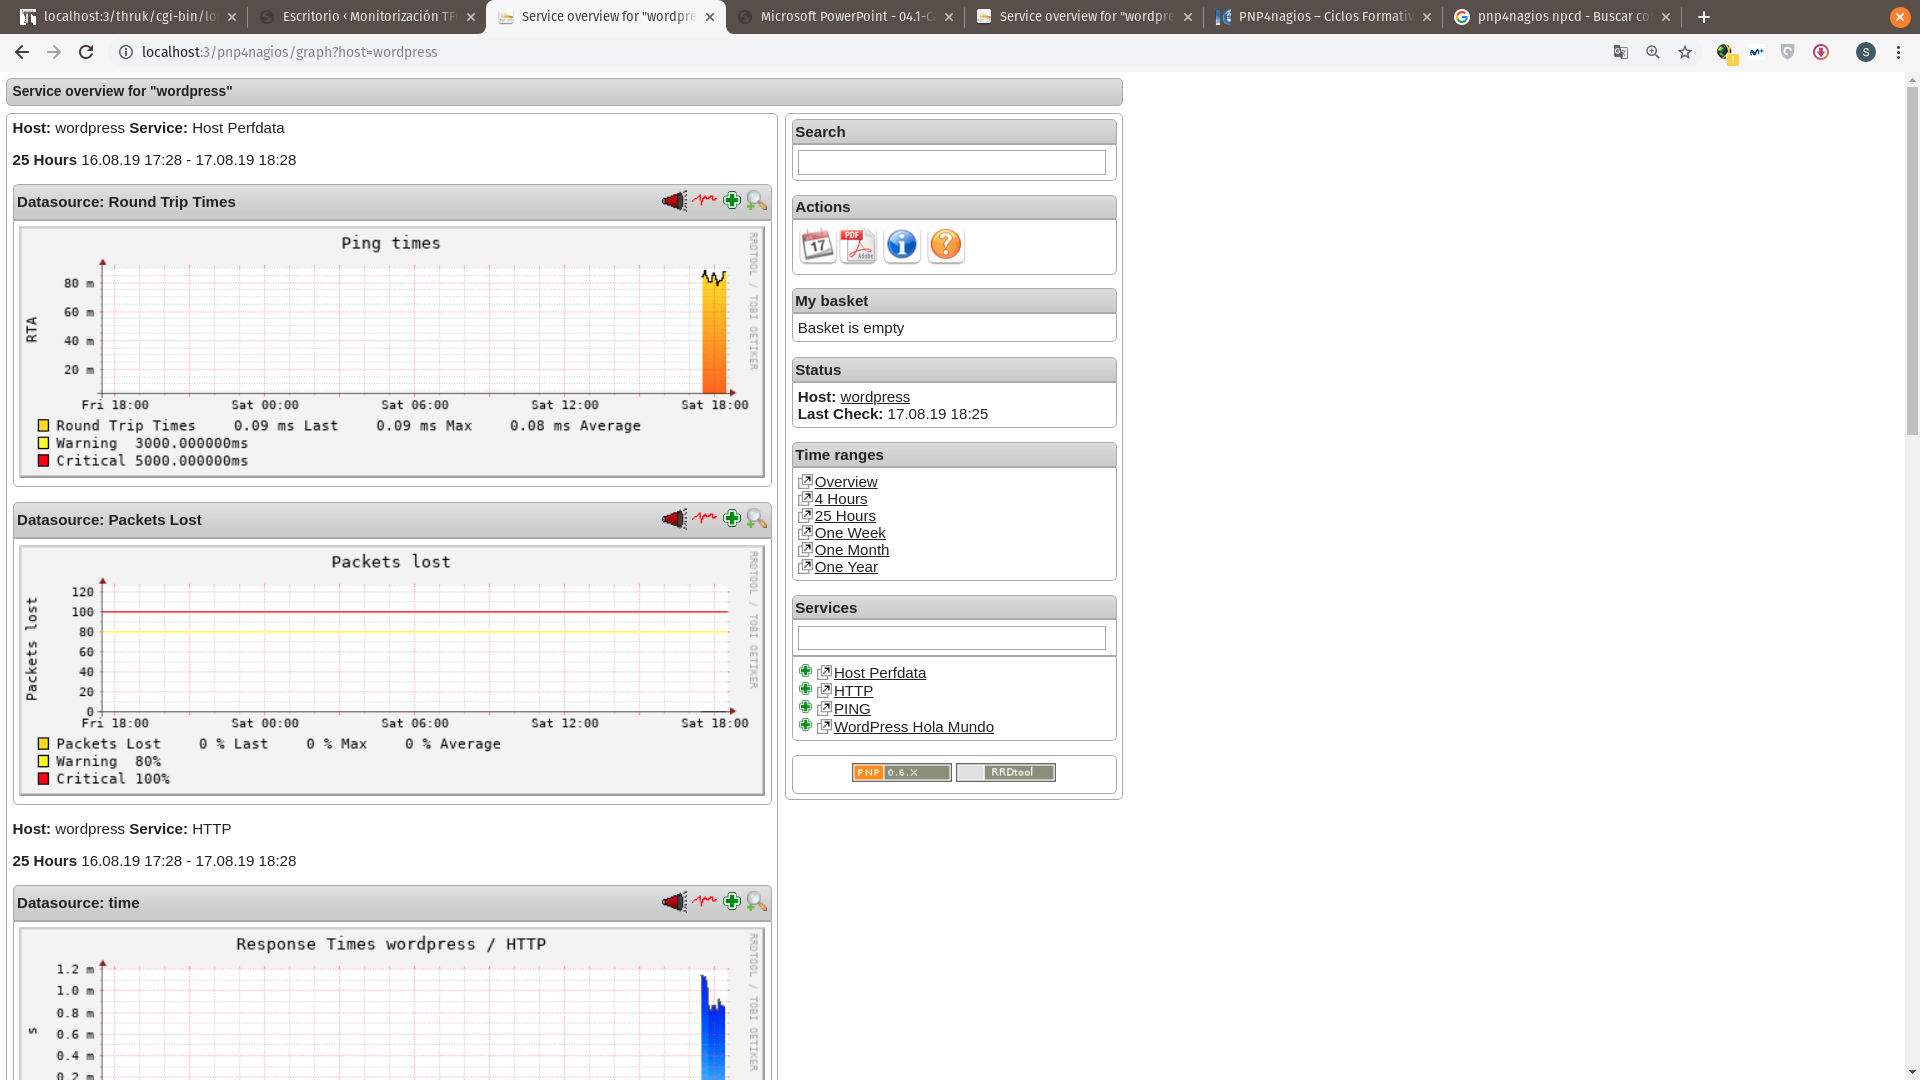
\includegraphics[scale=0.2]{imagenes/modelado/pnp4nagioscaptura.png}
	\caption{Estructura de PNP4Nagios} \label{pnp4nagios_estructura}
\end{figure}
\newpage
\subsection{Exportación de los datos a formato CSV}
Como ya tenemos todo para poder generar los datos, vamos a hacer uso de la herramienta que incluye PNP4Nagios para exportar en CSV, estos datos generados son los correspondientes a los datos generados por los servicios creados en el capítulo \ref{ch:carga_cliente}, donde realizábamos el servicio para comprobar \textbf{HTTP} y \textbf{PING}. 
Para ello la API \cite{exportcsv} nos ofrece la forma de exportación a CSV de la siguiente forma:
\url{/pnp4nagios/xport/<format>?host=<hostname>&srv=<servicedesc>}.
Donde:
\begin{itemize}
	\item \textbf{$<format>$} especifica el formato de exportación, teniéndose la opción de XML, JSON y CSV.
	\item \textbf{$<hostname>$} especificaremos el nombre del host, en este caso introducimos el nombre \textbf{wordpress}.
	\item \textbf{$<servicedesc>$} especificaremos el servicio que queremos exportar su información.	
\end{itemize}
Como queremos obtener la información de rendimiento del análisis de \textbf{HTTP} y \textbf{PING} solo tendremos que acceder a las siguientes direcciones:
\url{http://localhost:3/pnp4nagios/xport/CSV?host=wordpress&srv=PING}
\url{http://localhost:3/pnp4nagios/xport/CSV?host=wordpress&srv=HTTP}
Al acceder a estas dos direcciones obtendremos las tablas \ref{http_tabla} y \ref{ping_tabla} encontradas en el Anexo \ref{ch:anexo}.
Esta tabla se ha realizado con la toma de datos durante treinta minutos, durante este tiempo el sistema se encarga de mandar peticiones de tipo \textbf{HTTP} a la ruta /, obteniendo su tiempo de respuesta y el tamaño de los paquetes procesados. En el caso de la realización de las pruebas para el servicio \textbf{PING} comprueba durante treinta minutos la pérdida de paquetes y el tiempo RTA generado cuando se realiza una llamada al comando ping al host wordpress.
Esto queda quedará generado de la siguiente forma con el complemento \textbf{PNP4NAgios} en las figuras \ref{httppnp4nagios} y \ref{pingpnp4nagios}.
\newpage
\begin{figure}[H]
	\centering
	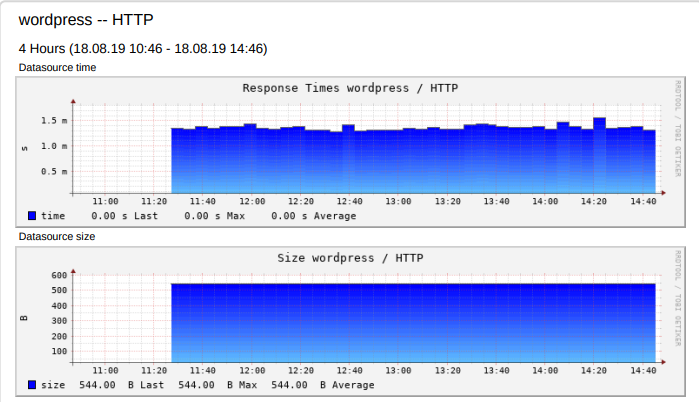
\includegraphics[scale=0.5]{imagenes/modelado/http.png}
	\caption{HTTP en interfaz PNP4Nagios} \label{httppnp4nagios}
\end{figure}
\begin{figure}[H]
	\centering
	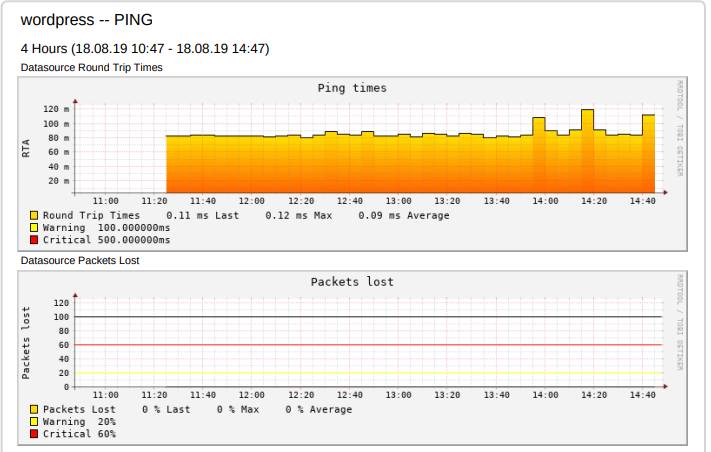
\includegraphics[scale=0.5]{imagenes/modelado/ping.png}
	\caption{PING en interfaz PNP4Nagios} \label{pingpnp4nagios}
\end{figure}
\newpage
Si pasamos a la generación de gráficos con los resultados obtenidos podemos obtener los siguientes gráficos:
\begin{figure}[H]
	\centering
	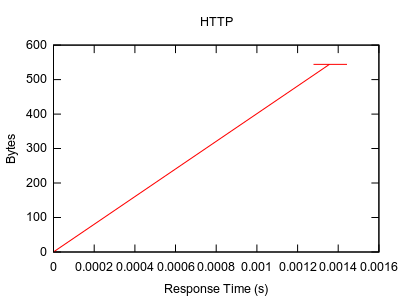
\includegraphics[scale=0.7]{valores_obtenidos/HTTP.png}
	\caption{Gráfica del servicio HTTP} \label{grafica_http}
\end{figure}
\begin{figure}[H]
	\centering
	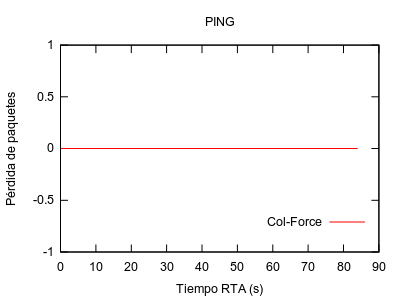
\includegraphics[scale=0.7]{valores_obtenidos/PING.png}
	\caption{Gráfica del servicio PING} \label{grafica_ping}
\end{figure}
En el capítulo \ref{ch:conclusion} se realizará un conclusión con los resultados obtenidos en el análisis de rendimiento de nuestro sistema.
\newpage